\documentclass[a4paper, 12pt, oneside]{book}
\usepackage[margin=3cm, bindingoffset=1cm]{geometry}
\linespread{1.5}
\usepackage[style=authoryear]{biblatex}
\addbibresource{bib.bib}
\usepackage{float}
\usepackage{csquotes}
\usepackage{subfig}
\usepackage{graphicx}
\usepackage{indentfirst}
\usepackage{fancyhdr}
\usepackage[english, italian]{babel}
\setlength{\parindent}{1cm}
\setlength{\headheight}{15pt}
\usepackage{amsthm}
\usepackage{amssymb}
\newtheoremstyle{example}{}{}{}{}{\bfseries}{\smallskip}{\newline}{}
\theoremstyle{example}
\newtheorem{example}{Esempio}[subsection]
\usepackage{float}
\usepackage[hidelinks]{hyperref}
\usepackage{orcidlink}

\usepackage{tikz}
\usetikzlibrary{shapes,trees}
\usetikzlibrary{graphs}

\pagestyle{fancy}
\renewcommand{\chaptermark}[1]{\markboth{\thechapter.\ \uppercase{#1}}{}}
\fancyhf{}
\fancyhead[C]{\textbf{\leftmark}}
\fancyfoot[C]{\thepage}
\renewcommand{\headrulewidth}{1pt}
\renewcommand{\footrulewidth}{1pt}
\usepackage[Conny]{fncychap}
\usepackage[style=altlist, nonumberlist, numberedsection, acronym, toc]{glossaries}
\selectlanguage{italian}

\title{Appunti Metodi Matematici per l'Informatica}
\author{Oleg Bilovus, \orcidlink{0000-0001-6285-5344}}
\date{Gennaio 2022}

\begin{document}
\begin{titlepage}
    \begin{center}
        \LARGE{\uppercase{Università degli Studi di Salerno}}\\
        \vspace{5mm}
        %Dipartimento
    	\uppercase{\normalsize Dipartimento di Informatica }\\
    \end{center}
    \begin{figure}[H]
        \centering
        
\includegraphics[width=0.35\textwidth]{cover/logo_unisa.png}
    \end{figure}
    
    \begin{center}
        %Corso di Laurea
    	\normalsize{ Corso di Laurea in Informatica }\\
    	\vspace{15mm}
    	%Titolo
        {\LARGE{\bf Appunti Metodi Matematici per l'Informatica}}\\
    	\vspace{3mm}
    \end{center}
    
    \vspace*{\fill}
    \noindent
    \hfill
    \begin{minipage}[t]{0.4\textwidth}\raggedleft
        %Candidato
    	{\large{Autore: \\ \bf \orcidlink{0000-0001-6285-5344} Oleg BILOVUS \\Mat. 0512105721}}
    \end{minipage}
    
    \vspace*{\fill}
    
    %Anno Accademico
    \centering{\large \uppercase{ Anno Accademico 2020/2021 }}

\end{titlepage}


\frontmatter
\chapter*{Abstract}
Gli appunti sono molto brevi e sintetici in quanto non sono pensati allo studio della materia, bensì al ripasso.
Gli appunti possono contenere errori, quindi non sono da considerare veritieri.



\tableofcontents
\clearpage

\mainmatter
\part{Logica, insiemi e dimostrazioni}
\label{par:first}

\chapter{Logica proposizionale}
\label{cha:logica_proposizionale}
\section{Perché studiare la logica proposizionale}
La materia insegna a distinguere quelle che sono delle proposizioni, ossia che hanno valore \textbf{True} \underline{\textit{oppure}} \textbf{False}, e quelle che invece non lo sono.

La frase \emph{Che bella giornata} non è una proposizione, in quanto essa può essere sia True che False.

Allo stesso modo affermazioni matematiche del tipo $x + 2 = 5$ non è una proposizione in quanto il valore della \textit{x} può variare e con esso varia il valore di verità della proposizione in True o False.

Invece proposizioni del tipo \emph{La penna è sul tavolo} oppure $5 + 4 = 0$ sono proposizioni in quanto hanno un valore di verità univoco al momento della loro affermazione.

\section{Proposizioni}
\subsection{Semplici}
Le proposizioni semplici sono dette tali quando hanno un valore \textbf{T} o \textbf{F} e non sono usati connettivi logici.
\begin{example}
\emph{La televisione è accesa}
\end{example}
\begin{example}
$3 + 5 = 8$
\end{example}

\subsection{Composte}
Le proposizioni composte sono dette tali quando hanno un valore \textbf{T} o \textbf{F} e sono usati connettivi logici.
\begin{example}
\emph{Laura fa i compiti \textbf{e} ascolta la musica}
\end{example}
\begin{example}
\emph{Se domani piove \textbf{allora} prenderò l'ombrello}
\end{example}

\section{Connettivi logici}

\subsection{NOT}
Il connettivo logico $\neg$ ha valore \textbf{T} se e solo se la proposizione \textit{p} ha valore \textbf{F}, e ha valore \textbf{F} se e solo se la proposizione \textit{p} ha valore \textbf{T}.

\begin{table}[H]
    \centering
    \caption{\label{tab:true_table_NOT}Tabella di verità del connettivo logico NOT.}
    \begin{tabular}{|c || c ||} 
     \hline
     \textit{p} & $\neg p$ \\
     \hline\hline
     T & F \\ 
     \hline
     F & T \\
     \hline
    \end{tabular}
\end{table}

\subsection{AND}
Il connettivo logico \textbf{$\wedge$} ha valore \textbf{T} se e solo se entrambe le proposizioni \textit{p} e \textit{q} hanno valore \textbf{T}, se una delle due è \textbf{F} allora il valore della proposizione è \textbf{F}.

\begin{table}[H]
    \centering
    \caption{\label{tab:true_table_AND}Tabella di verità del connettivo logico AND.}
    \begin{tabular}{|c | c || c ||} 
     \hline
     \textit{p} & \textit{q} & $p \wedge q$ \\
     \hline\hline
     T & T & T \\ 
     \hline
     T & F & F \\
     \hline
     F & T & F \\
     \hline
     F & F & F \\
     \hline
    \end{tabular}
\end{table}

\subsection{OR}
Il connettivo logico \textbf{$\vee$} ha valore \textbf{T} se e solo se una delle proposizioni \textit{p} o \textit{q} ha valore \textbf{T}, se sono entrambe \textbf{F} allora il valore della proposizione è \textbf{F}.

\begin{table}[H]
    \centering
    \caption{\label{tab:true_table_OR}Tabella di verità del connettivo logico OR.}
    \begin{tabular}{|c | c || c ||} 
     \hline
     \textit{p} & \textit{q} & $p \vee q$ \\
     \hline\hline
     T & T & T \\ 
     \hline
     T & F & T \\
     \hline
     F & T & T \\
     \hline
     F & F & F \\
     \hline
    \end{tabular}
\end{table}

\subsection{XOR}
Il connettivo logico \textbf{$\oplus$} ha valore \textbf{T} se e solo se una delle le proposizioni \textit{p} o \textit{q} ha valore \textbf{T} ma non entrambe, se sono entrambe \textbf{F} o \textbf{T} allora il valore della proposizione è \textbf{F}.

\begin{table}[H]
    \centering
    \caption{\label{tab:XOR}Tabella di verità del connettivo logico XOR.}
    \begin{tabular}{|c | c || c ||} 
     \hline
     \textit{p} & \textit{q} & $p \oplus q$ \\
     \hline\hline
     T & T & F \\ 
     \hline
     T & F & T \\
     \hline
     F & T & T \\
     \hline
     F & F & F \\
     \hline
    \end{tabular}
\end{table}

\subsection{Implicazione}
Il connettivo logico \textbf{$\implies$} ha valore \textbf{F} se e solo se la proposizione \textit{p} ha valore \textbf{T} e la proposizione \textit{q} ha valore \textbf{F}, altrimenti il valore della proposizione è \textbf{T}.

\begin{table}[H]
    \centering    
    \caption{\label{tab:true_table_implies}Tabella di verità del connettivo logico Implicazione.}
    \begin{tabular}{|c | c || c ||} 
     \hline
     \textit{p} & \textit{q} & $p \implies q$ \\
     \hline\hline
     T & T & T \\ 
     \hline
     T & F & F \\
     \hline
     F & T & T \\
     \hline
     F & F & T \\
     \hline
    \end{tabular}
\end{table}

\subsection{Equivalenza}
Il connettivo logico \textbf{$\iff$} ha valore \textbf{T} se e solo se la proposizione \textit{p} e la proposizione \textit{q} hanno valori uguali, altrimenti il valore della proposizione è \textbf{F}.

\begin{table}[H]
    \centering
    \caption{\label{tab:true_table_iff}Tabella di verità del connettivo logico Equivalenza.}
    \begin{tabular}{|c | c || c ||} 
     \hline
     \textit{p} & \textit{q} & $p \iff q$ \\
     \hline\hline
     T & T & T \\ 
     \hline
     T & F & F \\
     \hline
     F & T & F \\
     \hline
     F & F & T \\
     \hline
    \end{tabular}
\end{table}

\section{Equivalenza logica}
Due proposizioni composte \textit{p} e \textit{q} si dicono equivalenti logicamente se e solo se hanno la stessa tabella di verità e si indica con \textbf{p $\equiv$ q}.\\
\textbf{N.B:} $\equiv$ non è un connettivo logico. \\
\textbf{N.B:} $\equiv$ e $\iff$ sono diversi. \\
\textbf{N.B:} Non si usa il simbolo $=$ per esprimere l'equivalenza logica, ma si usa il simbolo $\equiv$.

\subsection{Tautologia}
La tautologia è una proposizione composta sempre \textbf{True}, ossia tutte \textbf{T} nella colonna della proposizione composta, qualsiasi sia il valore delle proposizioni elementari che la compongono. \\
\begin{table}[H]
    \centering    
    \caption{\label{tab:true_table_tautologia}Tabella di verità della tautologia $(p \wedge q) \implies (p \vee q)$.}
    \begin{tabular}{|c | c | c | c || c ||} 
     \hline
     \textit{p} & \textit{q} & $p \wedge q$ & $p \vee q$ & $(p \wedge q) \implies (p \vee q)$ \\
     \hline\hline
     T & T & T & T & T \\ 
     \hline
     T & F & F & T & T \\
     \hline
     F & T & F & T & T \\
     \hline
     F & F & F & F & T \\
     \hline
    \end{tabular}
\end{table}

\subsection{Contraddizione}
La contraddizione è una proposizione composta sempre \textbf{False}, ossia tutte \textbf{F} nella colonna della proposizione composta, qualsiasi sia il valore delle proposizioni elementari che la compongono.
\begin{table}[H]
    \caption{\label{tab:true_table_contraddizione}Tabella di verità della contraddizione $p \wedge \neg p$.}
    \centering
    \begin{tabular}{|c | c || c ||} 
     \hline
     \textit{p} & $\neg p$ & $p \wedge \neg p$ \\
     \hline\hline
     T & F & F \\ 
     \hline
     F & T & F \\
     \hline
    \end{tabular}
\end{table}

\section{Inverso, opposto e contronominale}
\subsection{Inverso}
Inverso di $p \implies q$ è $q \implies p$ \\
$p \implies q \not\equiv q \implies p$
\begin{table}[H]
    \centering    
    \caption{\label{tab:true_table_inverso}Tabella di verità di $p \implies q \not\equiv q \implies p$.}
    \begin{tabular}{|c | c | c || c ||} 
     \hline
     \textit{p} & \textit{q} & $p \implies q$ & $q \implies p$ \\
     \hline\hline
     T & T & T & T\\ 
     \hline
     T & F & F & T\\
     \hline
     F & T & T  & F\\
     \hline
     F & F & T & T \\
     \hline
    \end{tabular}
\end{table}
\begin{example}
\emph{Se domani piove \textbf{allora} prenderò l'ombrello} \\
Inverso: \emph{Prenderò l'ombrello \textbf{se} domani piove}
\end{example}

\subsection{Opposto}
Opposto di $p \implies q$ è  $\neg p \implies \neg q$ \\
$p \implies q \not\equiv \neg p \implies \neg q$
\begin{table}[H]
    \centering    
    \caption{\label{tab:true_table_opposto}Tabella di verità di $p \implies q \not\equiv \neg p \implies \neg q$.}
    \begin{tabular}{|c | c | c | c | c || c ||} 
     \hline
     \textit{p} & \textit{q} & $\neg p$ & $\neg q$ & $p \implies q$ & $\neg p \implies \neg q$ \\
     \hline\hline
     T & T & F & F & T & T\\ 
     \hline
     T & F & F & T & F & T\\
     \hline
     F & T & T & F & T & F\\
     \hline
     F & F & T & T & T & T\\
     \hline
    \end{tabular}
\end{table}
\begin{example}
\emph{Se domani piove \textbf{allora} prenderò l'ombrello} \\
Opposto: \emph{Se domani non piove \textbf{allora} non prenderò l'ombrello}
\end{example}

\subsection{Contronominale}
Contronominale di $p \implies q$ è  $\neg q \implies \neg p$ \\
$p \implies q \equiv \neg p \implies \neg q$
\begin{table}[H]
    \centering    
    \caption{\label{tab:true_table_contronominale}Tabella di verità di $p \implies q \equiv \neg p \implies \neg q$.}
    \begin{tabular}{|c | c | c | c | c || c ||} 
     \hline
     \textit{p} & \textit{q} & $\neg p$ & $\neg q$ & $p \implies q$ & $\neg q \implies \neg p$ \\
     \hline\hline
     T & T & F & F & T & T\\ 
     \hline
     T & F & F & T & F & F\\
     \hline
     F & T & T & F & T & T\\
     \hline
     F & F & T & T & T & T\\
     \hline
    \end{tabular}
\end{table}
\begin{example}
\emph{Se domani piove \textbf{allora} prenderò l'ombrello} \\
Contronominale: \emph{Non prenderò l'ombrello \textbf{se} domani non piove}
\end{example}

\subsection{Osservazione: l'inverso è equivalente logicamente all'opposto}
Dalla \autoref{tab:true_table_inverso} e dalla \autoref{tab:true_table_opposto} si ha che $q \implies p \equiv \neg p \implies \neg q$
\begin{table}[H]
    \centering    
    \caption{\label{tab:true_table_inverso_eqlogic_opposto}Tabella di verità di $q \implies p \equiv \neg p \implies \neg q$.}
    \begin{tabular}{|c | c | c | c | c || c ||} 
     \hline
     \textit{p} & \textit{q} & $\neg p$ & $\neg q$ & $q \implies p$ & $\neg p \implies \neg q$ \\
     \hline\hline
     T & T & F & F & T & T\\ 
     \hline
     T & F & F & T & T & T\\
     \hline
     F & T & T & F & F & F\\
     \hline
     F & F & T & T & T & T\\
     \hline
    \end{tabular}
\end{table}

\section{Equivalenze logiche note}
\subsection{Leggi di De Morgan}
\label{subs:de_morgan_laws}
\begin{itemize}
    \item $\neg(p \wedge q) \equiv \neg p \vee \neg q$
    \item $\neg(p \vee q) \equiv \neg p \wedge \neg q$
    \item $p \implies q \equiv \neg p \vee q$
    \item $\neg(p \implies q) \equiv \neg(\neg p \vee q) \equiv p \wedge \neg q$
\end{itemize}

\subsection{Equivalenze più usate}
\begin{itemize}
    \item $\neg(\neg p) \equiv p$
    \item $p \vee (q \wedge r) \equiv (p \vee q) \wedge (p \vee r)$
    \item $p \wedge (q \vee r) \equiv (p \wedge q) \vee (p \wedge r)$
    \item $(x < y < z) \equiv (x < y) \wedge (y < z)$
    \item $p \iff q \equiv (p \implies q) \wedge (q \implies p) \equiv (\neg p \vee q) \wedge (\neg q \vee p)$
\end{itemize}

\subsection{Altre equivalenze}
\begin{itemize}
    \item $p \wedge T \equiv p$
    \item $p \vee F \equiv p$
    \item $p \vee T \equiv T$
    \item $p \wedge F \equiv F$
    \item $p \vee p \equiv p$
    \item $p \wedge p \equiv p$
    \item $p \vee \neg p \equiv T$
    \item $p \wedge \neg p \equiv F$
\end{itemize}


\chapter{Logica predicativa}
\label{cha:logica_predicativa}
\section{Predicato}
Esprime una proprietà che un oggetto di un gruppo può avere o non avere o relazioni tra gli oggetti di un gruppo.
\begin{example}
$P(x, y)$ \textit{x} ama \textit{y} \\
\emph{Luca ama Laura}
\end{example}

Il predicato \textit{P} è una funzione con dominio l'universo del discorso e codominio il valore \textbf{T} o \textbf{F}.

\section{Quantificatori}
Essi vengono usati per esprime una proprietà su un gruppo di oggetti o l'esistenza di un oggetto con una proprietà in un gruppo.

\subsection{Universale}
Il quantificatore $\forall$ viene usato per esprimere una proprietà su un gruppo di oggetti. Per essere \textbf{T}, tutti gli oggetti nel dominio devono rispettare le proprietà.
\begin{example}
\emph{Tutti i laureati in informatica hanno fatto l'esame di MMI} \\
$P(x)$, \textit{x} è laureato in informatica \\
$Q(x)$, \textit{x} ha fatto l'esame di MMI \\
Dominio di \textit{x} sono tutti gli umani \\
$\forall xP(x) \implies Q(x)$
\end{example}

\textbf{N.B:} Se $\forall xP(x)$ è falso, ciò \underline{non} significata che tutti gli oggetti del dominio di \textit{x} non rispettino la proprietà \textit{P}, ma che esiste almeno un oggetto che non rispetta le proprietà.

\subsection{Esistenziale}
Il quantificatore $\exists$ viene usato per esprime l'esistenza di un oggetto con una determinata proprietà in un gruppo di oggetti. Affinché sia \textbf{T}, deve esistere almeno un oggetto che rispetti le proprietà.
\begin{example}
\emph{Alcuni laureati in informatica hanno fatto l'esame di programmazione avanzata} \\
$P(x)$, \textit{x} è laureato in informatica \\
$Q(x)$, \textit{x} ha fatto l'esame di programmazione avanzata \\
Dominio di \textit{x} sono tutti gli umani \\
$\exists xP(x) \wedge Q(x)$
\end{example}

\subsection{Dominio vuoto}
Se il dominio del predicato $P(x)$ è $\emptyset$, i quantificatori hanno i seguenti comportamenti: 
\begin{itemize}
    \item $\forall xP(x)$: è \textbf{T} in quanto non si può trovare un controesempio per dimostrare che è \textbf{F}.
    \item $\exists xP(x)$ è \textbf{F} in quanto non si può trovare un esempio per dimostrare che è \textbf{T}.
\end{itemize}

\subsection{Cambio dominio}
Se si cambia il dominio di un predicato, il valore di verità dell'intera proposizione può cambiare totalmente.
\begin{example}
\emph{Alcuni laureati in informatica hanno fatto l'esame di programmazione avanzata} \\
$P(x)$, \textit{x} ha fatto l'esame di programmazione avanzata \\
Dominio di \textit{x} tutti i laureati in informatica.
Allora avremmo che $\exists xP(x)$ è \textbf{T}. \\
Se cambiamo il dominio di \textit{x} in tutti i laureati di filosofia, avremmo che  $\exists xP(x)$ è \textbf{F}.
\end{example}

\subsection{Quantificatori innestati}
I quantificatori $\forall$ e $\exists$ si possono combinare tra di loro per formare predicati più complessi.
\begin{example}
\emph{Ogni figlio ha una madre} \\
$P(x)$, \textit{x} è un figlio \\
$Q(x)$, \textit{x} è una madre \\
$R(x, y)$, \textit{x} è figlio di \textit{y} \\
Dominio di \textit{x} e \textit{y} sono tutti gli umani \\
$\forall x \exists y \mid R(x, y) \wedge P(x) \wedge Q(y)$
\end{example}
\begin{example}
\emph{Ognuno apprezza qualcuno} \\
$P(x, y)$, \textit{x} apprezza y \\
Dominio di \textit{x} e \textit{y} sono tutti gli umani \\
$\forall x \exists y \mid P(x, y)$
\end{example}

\subsection{Negazione quantificatori}
I quantificatori possono essere negati. La regola generale è che se il quantificatore è $\forall$, diventa $\exists$ e viceversa e poi si nega il predicato.
\begin{itemize}
    \item $\neg(\forall xP(x)) \equiv \exists x \neg P(x)$
    \item $\neg (\exists xP(x)) \equiv \forall x \neg P(x)$
\end{itemize}

\subsubsection{Negazione quantificatori innestati}
La regola generale è che si cambiano i quantificatori con il loro opposto e si nega il predicato.
\begin{example}
$\neg(\forall x(P(x) \implies Q(x))) \equiv$ \\
$\exists x \neg(P(x) \implies Q(x)) \equiv$ \\ 
$\exists x \neg(\neg P(x) \vee Q(x)) \equiv$ \\
$\exists x(P(x) \wedge \neg Q(x))$
\end{example}
\begin{example}
Negare il seguente predicato $\forall x(x > 0 \implies \exists y \mid (x \cdot y=1))$ \\
$\neg(\forall x(x > 0 \implies \exists y \mid (x \cdot y=1))) \equiv$ \\
Si può spostare $\exists y$ all'inizio, in quanto lo scope di y non cambierebbe e risulta più facile la negazione \\
$\neg(\forall x(x > 0 \implies \exists y \mid (x \cdot y=1))) \equiv$ \\
$\neg(\forall x \exists y(x > 0 \implies (x \cdot y=1))) \equiv$ \\
$\exists x \forall y \neg(x > 0 \implies (x \cdot y=1))) \equiv$ \\
$\exists x \forall y \neg(\neg (x > 0) \vee (x \cdot y=1)) \equiv$ \\
$\exists x \forall y((x > 0) \wedge \neg (x \cdot y=1)) \equiv$ \\
$\exists x \forall y((x > 0) \wedge (x \cdot y \neq 1))$
\end{example}

\subsection{Dominio finito}
Se il dominio del predicato è finito ed è presente un quantificatore, esso può essere anche rimosso a seconda del quantificatore e la proposizione continuerà ad avere lo stesso valore di verità.
\begin{example} Supponiamo che il dominio del predicato $P(x)$ abbia \textit{n} oggetti. Avremmo che le seguenti equivalenze sono \textbf{T}:
\begin{itemize}
    \item $\forall xP(x) \iff P(x_1) \wedge P(x_2) \wedge ... \wedge P(x_n)$
    \item $\exists xP(x) \iff P(x_1) \vee P(x_2) \vee ... \vee P(x_n)$
    \item Funzione proposizionale $Q(x, y)$ con dominio $\{1, 2\} \times \{1, 2\}$ \\
    $\exists x \forall y Q(x, y) \iff (Q(1,1) \wedge Q(1, 2)) \vee (Q(2,1) \wedge Q(2, 2))$
    \item Funzione proposizionale $Q(x, y)$ con dominio $\{1, 2\} \times \{1, 2\}$ \\
    $\forall x \exists y Q(x, y) \iff (Q(1, 1) \vee Q(1, 2)) \wedge (Q(2, 1) \vee Q(2, 2))$
\end{itemize}
\end{example}

\section{Insieme di verità}
L'insieme di verità di $P(x)$ è l'insieme degli elementi $x_i$ nel dominio di $P(x)$ tali che $P(x)$ è \textbf{T}.

In termini matematici l'insieme di verità rappresenta un sottoinsieme della controimmagine di $P(x)$ tale che $P(x)=$ \textbf{T} \\
Il codominio di $P(x)$ è $C=\{T, F\}$, sia $D$ il dominio di $P(x)$, $V$ l'insieme di verità di $P(x)$ e $A=\{T\}\subset C$. \\
Si ha che l'insieme di verità di $P(x)$ è $f^{-1}(A)=\{x\in D \mid P(x)=T\}=V$
\begin{figure}[H]
\centering
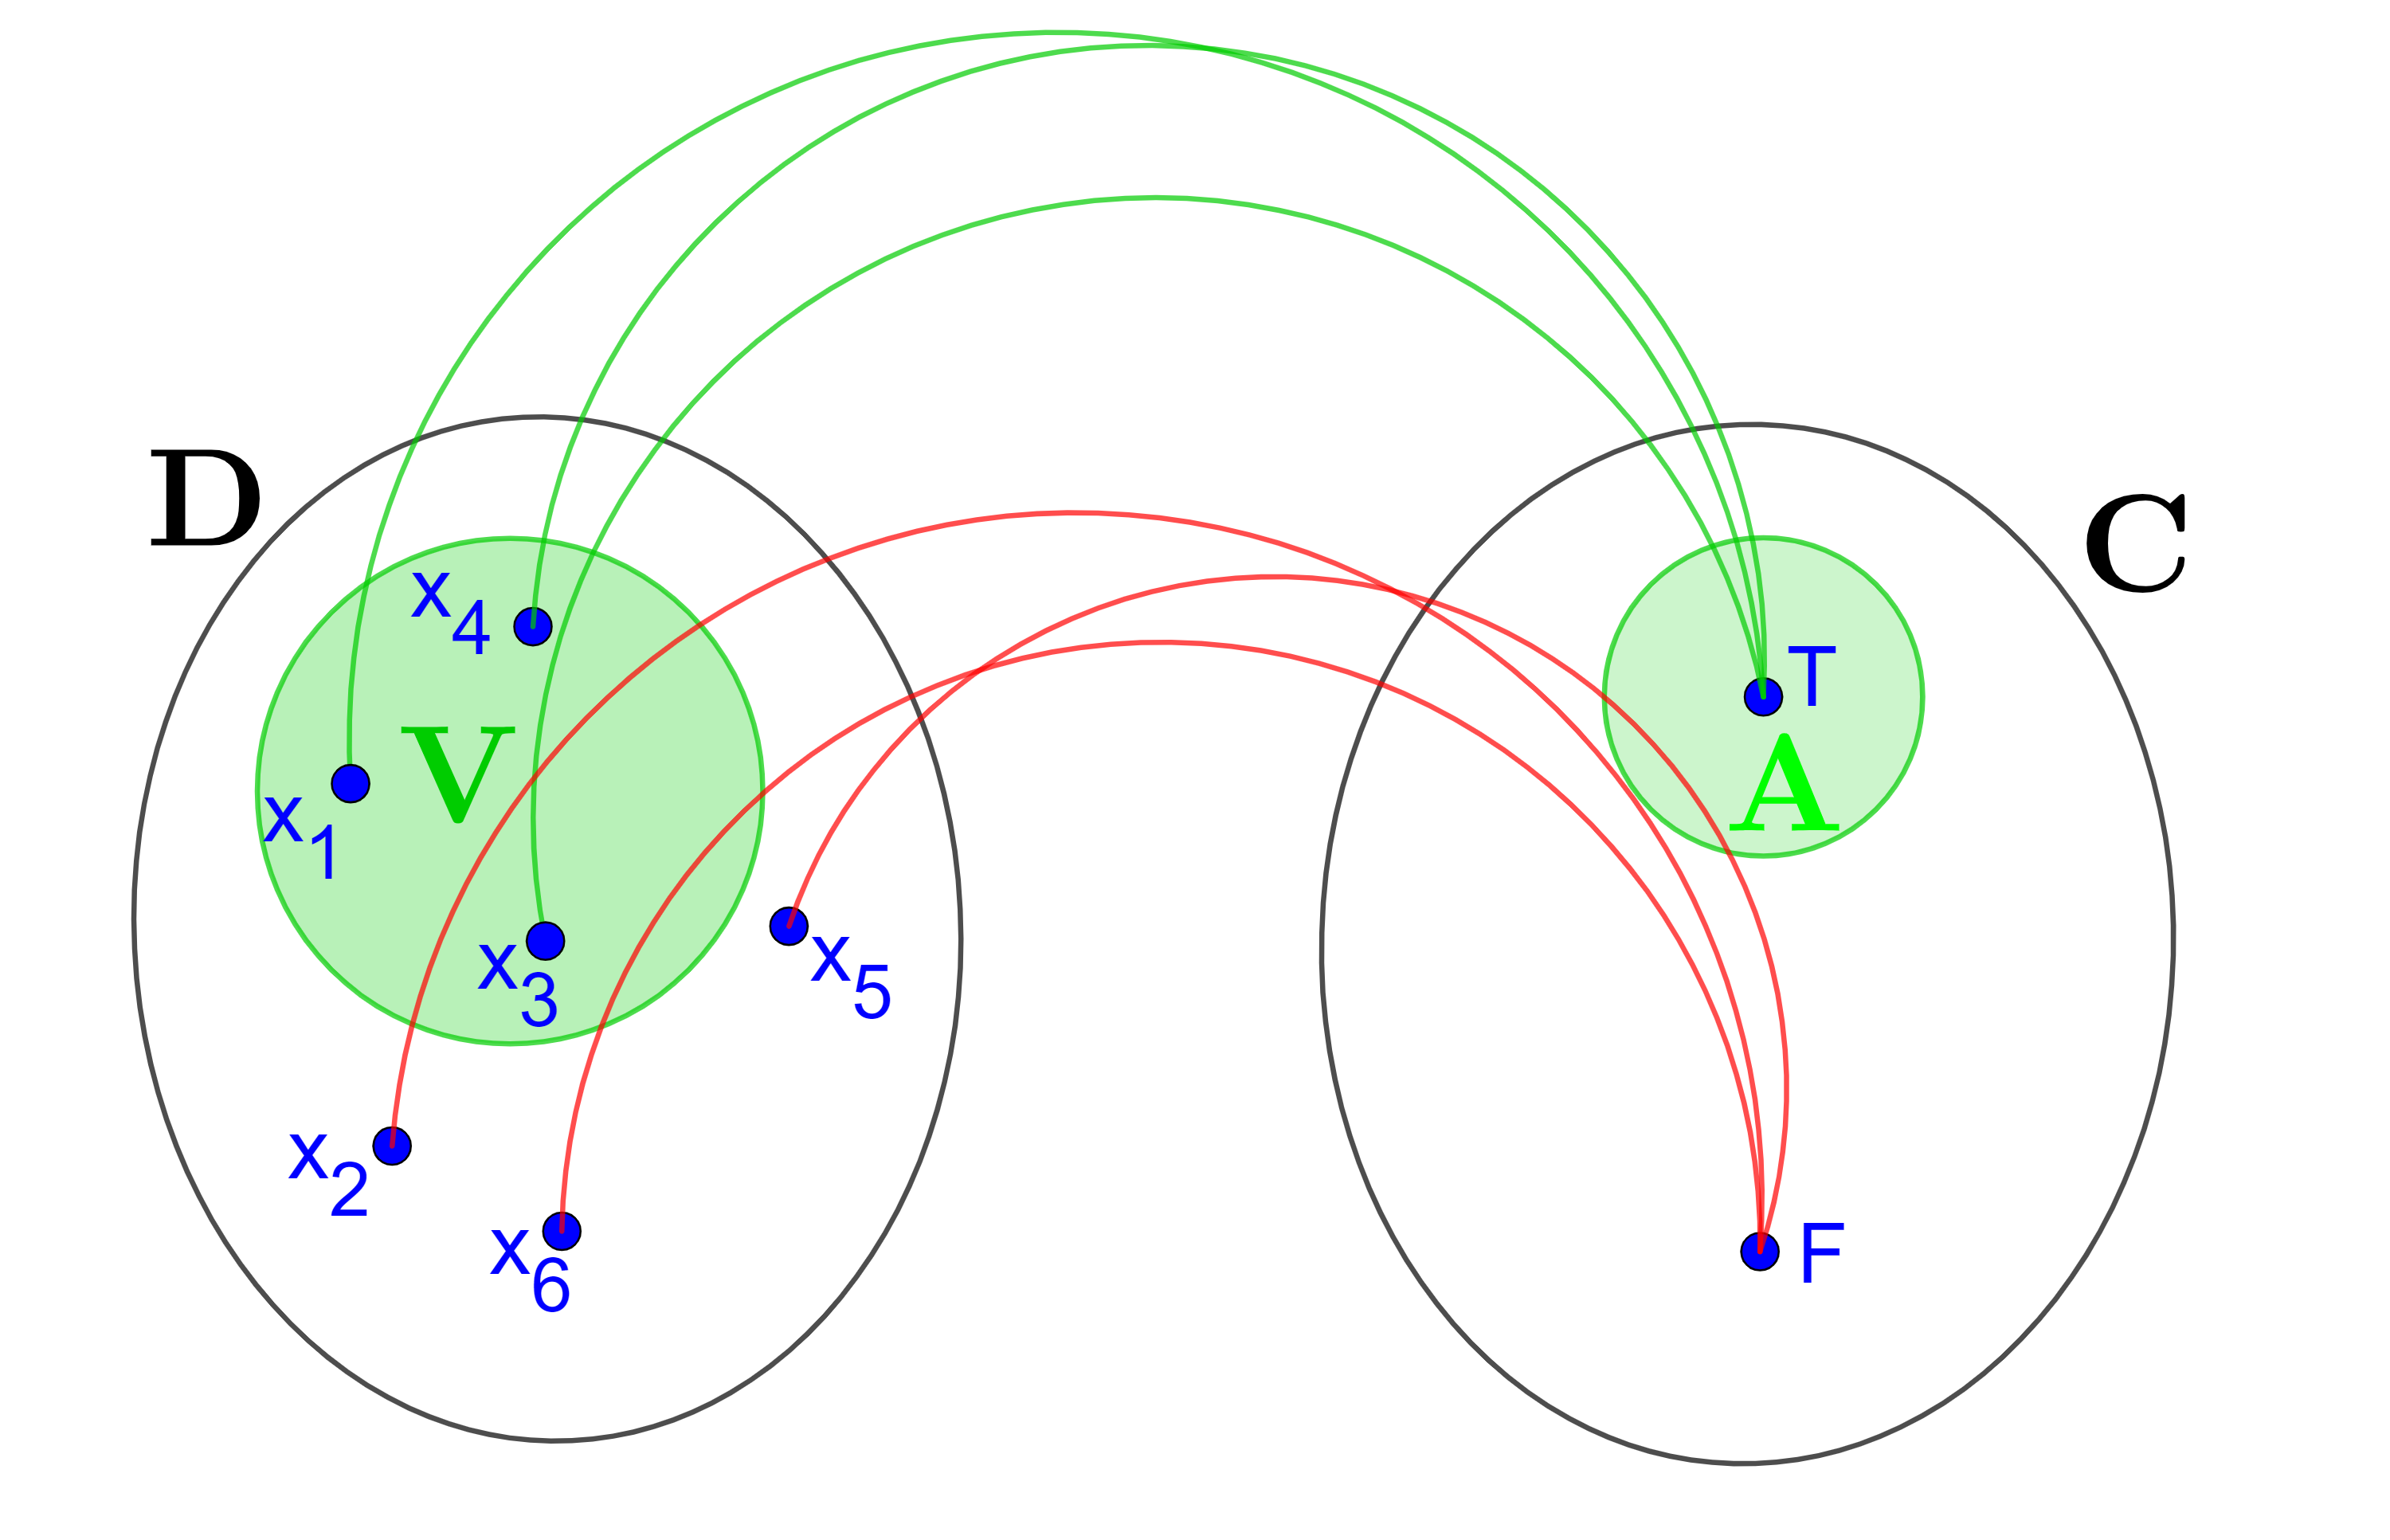
\includegraphics[scale=1.7]{chapters/logica_predicativa/figure_insieme_verita}
\caption{Rappresentazione grafica esempio di insieme di verità.}
\end{figure}

\chapter{Insiemi}
\label{cha:insiemi}
\begin{itemize}
    \item $A=B \iff A \subseteq B \wedge B \subseteq A$
    \item $A=B: \forall x(x \in A \iff x \in B) \equiv \forall x((x \in A \implies x \in B) \wedge (x \in B \implies x \in A))$
    \item $A \subseteq B: \forall x(x \in A \implies x \in B)$
    \item $A \not\subseteq B: \neg(\forall x(x \in A \implies x \in B) \equiv$ \\
        $\exists x \neg(x \in A \implies x \in B) \equiv$ \\
        $\exists x \neg(\neg (x \in A) \vee x \in B)) \equiv$ \\
        $\exists x(x \in A \wedge x \not\in B)$
    \item $\emptyset \in S: \forall x(x \in \emptyset \implies x \in S)$ è sempre \textbf{True} perché $x \in \emptyset$ è sempre falsa e dalla \autoref{tab:true_table_implies}, se $p$ è \textbf{F}, la proposizione è sempre \textbf{T}.
    \item $S \subseteq S: \forall x(x \in S \implies x \in S)$ è sempre \textbf{True} perché $p \implies p$ è una tautologia.
    \begin{table}[H]
    \centering
    \caption{\label{tab:true_table_p_implies_p}Tabella di verità di $p \implies p$.}
        \begin{tabular}{|c || c ||} 
         \hline
         \textit{p} & $p \implies p$ \\
         \hline\hline
         T & T \\ 
         \hline
         F & T \\
         \hline
        \end{tabular}
    \end{table}
    \item $A \subset B: \forall x(x \in A \implies x \in B) \wedge \exists y(y \in B \wedge y \not\in A)$
    \item $A \times B=\{(a, b)\mid a \in A \wedge b \in B\}$
\end{itemize}

\chapter{Dimostrazioni}
\label{cha:dimostrazioni}
\section{Dimostrazione diretta}
$p \implies q$
\begin{example}
\emph{Se \textit{n} è dispari allora $n^2$ è dispari.} \\
\textbf{Dimostrazione}: Sia \textit{n} un intero dispari. \\
$n^2=(2k+1)^2=4k^2+1+4k=2(2k^2+2k)+1$ \\
Quindi $n^2$ è dispari.
\end{example}

\section{Dimostrazione per contrapposizione}
\label{sec:dimostrazione_contrapposizione}

$\neg q \implies \neg p$ \\
Dalla \autoref{tab:true_table_contronominale} si ha che $\neg q \implies \neg p \equiv p \implies q$
\begin{example}
Se $3n+2$ è dispari allora \textit{n} è dispari. \\
\textbf{Contronominale}: Se \textit{n} è pari allora $3n+2$ è pari. \\
\textbf{Dimostrazione}: Sia n pari. \\
$3n+2=3(2k)+2=2(3k)+2=2(3k+1)$ \\
$2(3k+1)$ è sempre un numero pari in quanto $2 \cdot r, r \in \mathbb{R}$ è sempre pari. \\
Avendo dimostrato che $\neg q \implies \neg p$ è \textbf{True} e poiché $\neg q \implies \neg p \equiv p \implies q$, si ha che \emph{$3n+2$ è dispari allora \textit{n} è dispari} è \textbf{True}.
\end{example}

\section{Dimostrazione per assurdo o contraddizione}
$p \implies q$ è \textbf{T} quando $p \wedge \neg q$ è \textbf{F} \\
Si ricorda che dalle \nameref{subs:de_morgan_laws} si ha che $\neg (p \implies q) \equiv p \wedge \neg q$
\begin{table}[H]
    \centering    
    \caption{\label{tab:true_table_p_imp_q__p_and_not_q}Tabella di verità di $p \implies q$ e $p \wedge \neg q$.}
    \begin{tabular}{|c | c | c | c || c ||} 
     \hline
     \textit{p} & \textit{q} & $\neg q$ & $p \implies q$ & $p \wedge \neg q$ \\
     \hline\hline
     T & T & F & T & F \\ 
     \hline
     T & F & T & F & T \\
     \hline
     F & T & F & T & F \\
     \hline
     F & F & T & T & F \\
     \hline
    \end{tabular}
\end{table}
\begin{example}
\emph{Se $3n+2$ è dispari allora \textit{n} è dispari}. \\
\textbf{$p \wedge \neg q$}: $3n+2$ è dispari e \textit{n} è pari. \\
\textbf{Dimostrazione}: \\
$3n+2=3(2k)+2=2(3k+1)$ \\
Nella \nameref{sec:dimostrazione_contrapposizione} abbiamo visto che $2(3k+1)$ è sempre pari. Poiché $3n+2=2(3k+1)$ allora $3n+2$ è pari, ma avevamo detto che era dispari. Quindi è un assurdo e \textbf{$p \wedge \neg q$} è \textbf{F}, quindi $p \implies q$ è \textbf{T}, cioè \emph{Se $3n+2$ è dispari allora \textit{n} è dispari} è \textbf{T}.
\end{example}

\section{Dimostrazione banale o vuota}
$p \implies q$, \textit{p}=\textbf{F} allora dalla \autoref{tab:true_table_implies} $p \implies q$ è sempre \textbf{True}.

\section{Dimostrazione di equivalenza}
$p \iff q$ \\
Si dimostra $(p \implies q) \wedge (q \implies p)$

\section{Controesempio}
$\forall x P(x)$ \\
$\neg(\forall x P(x)) \equiv \exists x\neg P(x)$

\section{Prova di esistenza}
$\exists x P(x)$
\begin{itemize}
    \item Può essere costruttiva esibendo un elemento \textit{x} nel dominio per cui $P(x)$ è \textbf{True}.
    \item Può essere non costruttiva.
\end{itemize}

\section{Dimostrazione per casi}
$(p_1 \vee p_2 \vee ... \vee p_n) \implies q \equiv (p_1 \implies q) \vee (p_2 \implies q) \vee ... \vee (p_n \implies q)$

\section{Dimostrazione esaustiva}
<<TODO>>


\part{Ricorsione, principio induzione e relazioni di ricorrenze}
\label{par:second}

\chapter{Definizione funzioni ricorsivamente}
\label{cha:def_ric_funz}
\section{Funzione matematica in $\mathbb{N}$}
\textbf{Passo base}: Specificare il valore della funzione in $0$.

\textbf{Passo ricorsivo}: Definire la regola per ottenere il valore della funzione su un intero attraverso i valori della funzione su interi più piccoli.

\begin{example}
$f: \mathbb{N} \longrightarrow \mathbb{N}$ \\
\textbf{Passo Base}: $f(0) = 3$ \\
\textbf{Passo ricorsivo}: $f(n + 1) = 2f(n) + 3$
\end{example}

La funzione target, ad esempio $f(3)$, si può calcolare buttom up o top down.

\subsection{Calcolo buttom up}
Si parte dal \textbf{Passo base}, in quanto si conosce il valore della funzione e si arriva a ogni iterazione al valore della funzione target.
\begin{example}
$f(0) = 3 \\
f(1) = 2 \cdot 3 + 3 = 9 \\
f(2) = 2 \cdot 9 + 3 = 21 \\
f(3) = 2 \cdot 21 + 3 = 45$
\end{example}

\subsection{Calcolo top down}
Si parte dal target, ad esempio $f(3)$, e si scrive la sua funzione ricorsiva. Si scende fino al \textbf{Passo base} in quanto non si conosce il valore delle precedenti funzioni ricorsive. Arrivati al \textbf{Passo base}, si inizia a scrivere il valore delle funzioni che si conoscono a ritroso, in questo modo si arriverà al valore della funzione target.
\begin{example}
$f(3) = 2f(2) + 3 = 2 \cdot 21 + 3 = 45 \\
f(2) = 2f(1) + 3 = 2 \cdot 9 + 3 = 21 \\
f(1) = 2f(0) + 3 = 2 \cdot 3 + 3 = 9 \\
f(0) = 3$
\end{example}

\section{Dalla definizione ricorsiva alla funzione ricorsiva}
Per passare dalla definizione ricorsiva alla funzione ricorsiva bisogna scoprire il meccanismo ricorsivo. Lo si può fare calcolando il \textbf{Passo base}, la funzione in \textit{n}, cioè $f(n)$, e la funzione in $f(n + 1)$.

\textbf{N.B}: la funzione ricorsiva è $f(n + 1)$. \\
\textbf{N.B}: nella funzione ricorsiva $f(n + 1)$ ci deve essere sempre una chiamata a valori di funzioni precedenti a $f(n + 1)$, altrimenti non è una funzione ricorsiva.
\begin{example}
Fibonacci \\
\centerline{\textbf{Definizione ricorsiva}} \\
\textbf{Passo base}: $F_0 = F_1 = 1$ \\
\textbf{Passo ricorsivo}: $F_n = F_{n - 1} + F_{n - 2}, n \geq 2$ \\
\centerline{\textbf{Funzione ricorsiva}}
$f(0) = 1 \\
f(1) = 1 \\
f(n) = f(n - 1) + f(n - 2) \\ 
f(n + 1) = f((n + 1) - 1) + f((n + 1) - 2) = f(n) + f(n - 1)$ 
\end{example}

\begin{example}
$f: \mathbb{N} \longrightarrow \mathbb{N}$ \\
\centerline{\textbf{Definizione ricorsiva}} \\
$f(n) = a^n$ \\
\centerline{\textbf{Funzione ricorsiva}}
$f(0) = a^0 = 1 \\
f(n) = a^n \\ 
f(n + 1) = a^{n + 1} = a \cdot a^n = a \cdot f(n)$ \\
\textbf{N.B.}: Se avessimo scritto solamente $f(n + 1) = a^{n + 1} = a \cdot a^n$, non è corretto, in quanto non è una definizione ricorsiva poiché non vi sono chiamate ai valori delle funzioni precedenti a $f(n + 1)$.
\end{example}


\chapter{Definizione insiemi ricorsivamente}
\label{cha:def_ric_ins}
\section{Insiemi numerici}
Applicare il passo ricorsivo un paio di volte, capire cosa contiene l'insieme e darne la costruzione ricorsiva. La correttezza della costruzione ricorsiva sarà dimostrata successivamente con il \nameref{cha:principio_induzione}.
\begin{example}
\phantom{}
\centerline{\textbf{Definizione ricorsiva}}
\textbf{Passo base}: $1 \in A$ \\
\textbf{Passo ricorsivo}: Se $x \in A$, allora $x + 2 \in A$ \\ 
\centerline{\textbf{Costruzione ricorsiva}}
Applico il passo ricorsivo \\
$x = 1 \in A$, allora $x + 2 = 1 + 2 = 3 \in A$ \\
Applico il passo ricorsivo \\
$x = 3 \in A$, allora $x + 2 = 3 + 2 = 5 \in A$ \\

Si può notare che \textit{A} contiene i numeri dispari, quindi la sua costruzione ricorsiva è: $A = \{2n + 1 \mid n \geq 0, n \in \mathbb{N}\}$
\end{example}

\begin{example}
\phantom{}
\centerline{\textbf{Definizione ricorsiva}}
\textbf{Passo base}: $3 \in S$ \\
\textbf{Passo ricorsivo}: Se $x, y \in S$, allora $x + y \in S$ \\
\centerline{\textbf{Costruzione ricorsiva}}
Applico il passo ricorsivo \\
$x = 3 \in S, y = 3 \in S$, allora $x + y = 3 + 3 = 6 \in S$ \\
Applico il passo ricorsivo \\
$x = 6 \in S, y = 3 \in S$, allora $x + y = 6 + 3 = 9 \in S$ \\
Applico il passo ricorsivo \\
$x = 9 \in S, y = 3 \in S$, allora $x + y = 9 + 3 = 12 \in S$ \\
Applico il passo ricorsivo \\
$x = 9 \in S, y = 6 \in S$, allora $x + y = 9 + 6 = 15 \in S$ \\

Si può notare che \textit{S} contiene i numeri multipli di 3, quindi la sua costruzione ricorsiva è: $S = \{3n \mid n \geq 1, \in \mathbb{N}\}$
\end{example}

\begin{example}
\phantom{}
\centerline{\textbf{Definizione ricorsiva}}
\textbf{Passo base}: $1 \in T$ \\
\textbf{Passo ricorsivo}: Se $x \in T$, allora $3 \cdot x \in T$ \\
\centerline{\textbf{Costruzione ricorsiva}}
Applico il passo ricorsivo \\
$x = 1 \in T$, allora $3 \cdot x = 3 \cdot 1 = 3 \in T$ \\
Applico il passo ricorsivo \\
$x = 3 \in T$, allora $3 \cdot x = 3 \cdot 3 = 9 \in T$ \\
Applico il passo ricorsivo \\
$x = 9 \in T$, allora $3 \cdot x = 3 \cdot 9 = 27 \in T$ \\

Si può notare che \textit{T} contiene i numeri $3^n$, quindi la sua costruzione ricorsiva è: $T = \{3^n \mid n \in \mathbb{N}\}$
\end{example}

\chapter{Definizione stringhe ricorsivamente}
\label{cha:def_ric_str}
\section{Definizioni}
\begin{itemize}
    \item L'alfabeto $\Sigma$ è un insieme di simboli per creare stringhe.
    \item La stringa è una \textbf{sequenza} di simboli presi da un alfabeto $\Sigma$.
    \item $\lambda$ è la \textbf{stringa vuota} che non contiene simboli. $\lambda$ è una \textbf{stringa} e non un simbolo dell'alfabeto $\Sigma$, quindi $\lambda \not\in \Sigma$.
    \item $\Sigma^*$ è l'insieme di tutte le possibili stringhe sull'alfabeto $\Sigma$.
    \item L'insieme $\Sigma^*$ è infinito e $\lambda \in \Sigma^*$.
\end{itemize}

\section{Definizione ricorsiva di $\Sigma^*$}
\textbf{Passo base}: $\lambda \in \Sigma^*$

\textbf{Passo ricorsivo}: Se $w \in \Sigma^*$ e $x \in \Sigma$, allora $wx \in \Sigma^*$
\begin{example}
$\Sigma = \{0, 1\}$ \\
Dal \textbf{Passo base} si ha che $\lambda \in \Sigma^*$. Quindi al \textbf{Passo base} $\Sigma^*=\{\lambda\}$ \\
Applico il passo ricorsivo \\
$w = \lambda \in \Sigma^*, x = 0 \in \Sigma$, allora $wx = \lambda 0 = 0 \in \Sigma^*$. Quindi $\Sigma^*=\{\lambda, 0\}$ \\
Applico il passo ricorsivo \\
$w = \lambda \in \Sigma^*, x = 1 \in \Sigma$, allora $wx = \lambda 1 = 1 \in \Sigma^*$. Quindi $\Sigma^*=\{\lambda, 0, 1\}$ \\
Applico il passo ricorsivo \\
$w = 0 \in \Sigma^*, x = 0 \in \Sigma$, allora $wx = 00 \in \Sigma^*$. Quindi $\Sigma^*=\{\lambda, 0, 1, 00\}$ \\
Applico il passo ricorsivo \\
$w = 0 \in \Sigma^*, x = 1 \in \Sigma$, allora $wx = 01 \in \Sigma^*$. Quindi $\Sigma^*=\{\lambda, 0, 1, 00, 01\}$ \\
...
\end{example}

\section{Lunghezza di una stringa}
\textbf{Passo base}: $|\lambda| = 0$

\textbf{Passo ricorsivo}: Se $w \in \Sigma^*$ e $x \in \Sigma$, allora $|wx| = |w| + 1$

\begin{example}
$|abb| = |ab| + |b| = |a| + |b| + |b| = 1 + 1 + 1 = 3$
\end{example}

\section{Concatenazione di una stringa}
$u$ e $v$ due stringhe, la concatenazione di $u$ e $v$ è la stringa $u \cdot v$. Si indica anche semplicemente con $uv$ senza usare il $\cdot$ \\
\textbf{N.B}: $uv \neq vu$ \\
\textbf{Passo base}: Se $w \in \Sigma^*$, allora $w \lambda = w$ \\
\textbf{Passo ricorsivo}: Se $w_1, w_2 \in \Sigma^*$ e $x \in \Sigma$, allora $w_1 \cdot (w_2x) = (w_1 \cdot w_2)x \in \Sigma^*$
\begin{example}
$abb \cdot ab = abb \cdot (ab) = abba \cdot b = abbab$
\end{example}

\section{Potenza di una stringa}
\textbf{Passo base}: $w^0 = \lambda$

\textbf{Passo ricorsivo}: $w^{n + 1} = w^n \cdot w, \forall n \geq 0$
\begin{example}
$\{(aa)^i \mid 0 \leq i \leq 3\} = \{ \lambda, aa, aaaa, aaaaaa\}$
\end{example}
\begin{example}
$\{aa^i \mid 0 \leq i \leq 3\} = \{ \lambda, aa, aaa, aaaa\}$
\end{example}
\textbf{N.B}: $(aa)^i \neq aa^i$, $(aa)^2 = aaaa, aa^2 = aaa$

\section{Stringa palindroma}
\textbf{Passo base}: $\forall x \in \Sigma$ e $\lambda$ sono stringhe palindrome

\textbf{Passo ricorsivo}: Se $w$ è una stringa palindroma e $x \in \Sigma$, allora $xwx$ è una  stringa palindroma.
\begin{example}
$abba$ \\
Per il \textbf{Passo base} $a, b, \lambda$ sono stringhe palindrome \\
Applico il passo ricorsivo \\
$w = \lambda$ palindroma per il \textbf{Passo base} e $x = b \in \Sigma$, allora $xwx = b \lambda b = bb$ è una stringa palindroma. \\
Applico il passo ricorsivo \\
$w = bb$ palindroma per il passo ricorsivo precedente e $x = a \in \Sigma$, allora $xwx = abba$ è una stringa palindroma.
\end{example}

\section{Inversione di una stringa}
\textbf{Passo base}: $\lambda^R = \lambda$

\textbf{Passo ricorsivo}: Se $w \in \Sigma^*$ e $x \in \Sigma$, allora $(wx)^R = xw^R$

\begin{example}
$(abb)^R = b(ab)^R = bb(a)^R = bba$
\end{example}
\begin{example}
$a^R = (\lambda a)^R = a \lambda^R = a \lambda = a$
\end{example}

\section{Ulteriori definizioni di specifiche stringhe}
\subsection{Stringhe su $\{a, b\}$ di lunghezza pari}
\textbf{Passo base}: $\lambda \in S$

\textbf{Passo ricorsivo}: Se $w \in S$, allora $waa, wab, wba, wbb \in S$

\subsection{Stringhe pari su $\{a, b\}$ che iniziano con a}
\textbf{Passo base}: $aa, ab \in S$

\textbf{Passo ricorsivo}: Se $w \in S$, allora $waa, wab, wba, wbb \in S$

\subsection{Morfismo}
Prende in input $w \in \{a, b\}^* \setminus \lambda$ e sostituisce $a$ con $0$ e $b$ con $1$

\textbf{Passo base}: $change(a)=0$, $change(b)=1$

\textbf{Passo ricorsivo}: $change(wx)= \begin{cases} change(w)0, \text{ se } x=a \\ change(w)1, \text{ se } x=b \end{cases}$

\chapter{Definizione alberi radicati ricorsivamente}
\label{cha:def_ric_albero_radicato}
\section{Definizioni}
\begin{figure}[H]
    \centering
    \begin{tikzpicture}[
        scale=1.4, 
        every node/.style={draw=green, fill=green!20, circle, ultra thick, scale=1.4}, 
        edge from parent/.style={draw, very thick}, 
        ->
        ]
    \node[draw=red, fill=red!20]{1}
        child { node[draw=blue, fill=blue!20]{2}
            child { node {5} }
            child { node {6} }
        }
        child { node{3}
        }
        child {node[draw=blue, fill=blue!20] {4} 
            child { node {7} }
        };
    \end{tikzpicture}
    \caption{Esempio albero radicato.}
    \label{fig:example_albero_radicato}
\end{figure}

\begin{itemize}
    \item Un albero radicato per definizione ha \textcolor{red}{\textbf{una sola radice}}, nella \autoref{fig:example_albero_radicato} in questo caso è il \textcolor{red}{nodo 1}.
    \item Un albero radicato ha \textcolor{green}{\textbf{una o più foglie}}, nella \autoref{fig:example_albero_radicato} sono i \textcolor{green}{nodi 3, 5, 6 e 7}.
    \item Un albero radicato può avere \textcolor{blue}{\textbf{uno o più genitori/nodi interni}}, essi per definizione sono nodi che hanno almeno un figlio, cioè che non sono foglie, nella \autoref{fig:example_albero_radicato} sono i \textcolor{blue}{nodi 2, 4} e anche la radice \textcolor{red}{nodo 1} in questo caso è un genitore/nodo interno.
    \item Un albero radicato può essere rappresentato da una coppia di insiemi $T=(V, E)$. Prendiamo come esempio la \autoref{fig:example_albero_radicato}.
    \begin{itemize}
        \item $V$ rappresenta i nodi, detti anche vertici o dall'inglese \emph{\textbf{V}ertexes}. \\
        $V=\{1, 2, 3, 4, 5, 6, 7\}$. 
        \item $E$ rappresenta gli archi, dall'inglese \emph{\textbf{E}dges}. L'insieme è composto a sua volta da coppie di nodi \textit{(genitore, figlio)} dall'insieme $V$. \\
        $E \subset V \times V$\\
        $E=\{(1, 2), (1, 3), (1, 4), (2, 5), (2, 6), (4, 7)\}$. \\
        \textbf{Osservazione}: la radice compare solo a sinistra delle coppie in quanto è l'unico nodo che è solo genitore e non ha genitori. Le foglie invece compaiono solo a destra delle coppie poiché per definizione non hanno figli.
        \item Infine la coppia viene chiamata $T$, dall'inglese \emph{\textbf{T}ree}, cioè albero. \\
        $T=(\{1, 2, 3, 4, 5, 6, 7\},\{(1, 2), (1, 3), (1, 4), (2, 5), (2, 6), (4, 7)\})$. \\
    \end{itemize}
\end{itemize}

\section{Definizione ricorsiva}
\textbf{Passo base}: $T=(\{r\}, \{\emptyset\})$ è un albero radicato

\begin{figure}[H]
    \centering
    \begin{tikzpicture}[
        scale=1.4, 
        every node/.style={draw, circle, ultra thick, scale=1.4}
        ]
    \node{r};
    \end{tikzpicture}
    \caption{Passo base definizione ricorsiva albero radicato.}
    \label{fig:pb_def_ric_albero_radicato}
\end{figure}

\textbf{Passo ricorsivo}: Supponiamo che $T_1=(V_1, E_1), ..., T_n=(V_n, E_n)$ siano alberi radicati disgiunti, cioè $\displaystyle\bigcap^n_{i=1} V_i = \emptyset$ (gli alberi non hanno nodi in comune). Le respettive radici sono $r_1 \in V_1, ..., r_n \in V_n$.
Allora $T=(V, E)$ si ottiene ponendo come radice un nodo $r \not\in V_1 \cup ... \cup V_n$ e da $r$ si aggiunge un arco a ogni $r_1 \in V_1, ..., r_n \in V_n$. 

$V = \{r\} \cup V_1 \cup ... \cup V_n$

$E = \{(r, r_1), ..., (r, r_n)\} \cup E_1 \cup ... \cup E_n$ \\
$T = (V, E)$ è un albero radicato.

\begin{figure}[H]
    \centering
    \begin{tikzpicture}[
        scale=1.4, 
        every node/.style={draw, circle, ultra thick, scale=1.4, minimum size=0.8cm},
        edge from parent/.style={draw, very thick},
        norm/.style={draw=black},
        green_edge/.style={draw=green},
        ->
        ]
    \node{r}
        child[green_edge] { node[norm]{$r_1$}
            child[norm] { node[draw=none, label={270:$T_1$}]{...} }
        }
        child[green_edge] { node[norm]{...}
            child[norm] { node[draw=none, label={270:...}]{...} }
        }
        child[green_edge] { node[norm]{$r_n$}
            child[norm] { node[draw=none, label={270:$T_n$}]{...} }
        };
    \end{tikzpicture}
    \caption{Passo ricorsivo definizione ricorsiva albero radicato.}
    \label{fig:pr_def_ric_albero_radicato}
\end{figure}

\section{Numero di vertici}
\textbf{Passo base}: Se $T=(\{r\}, \emptyset)$, allora $|V|=1$

\textbf{Passo ricorsivo}: Se $T=(V, E)$ è un albero radicato costruito a partire dagli alberi $T_1=(V_1, E_1), ..., T_n=(V_n, E_n)$, allora $|V| = 1 + |V_1| + ... |V_n|$. \\
\textbf{N.B.}: L'$1$ rappresenta la radice $r \not\in V_1 \cup ... \cup V_n$, così come definito nel Passo ricorsivo della costruzione dell'albero radicato. Nella \autoref{fig:pr_def_ric_albero_radicato} è il vertice $r$.

\section{Numero di edges(archi)}
\textbf{Passo base}: Se $T=(\{r\}, \{\emptyset\})$, allora $|E| = 0$

\textbf{Passo ricorsivo}: Se $T=(V, E)$ è un albero radicato costruito a partire da $T_1=(V_1, E_1), ..., T_n=(V_n, E_n)$, allora $|E| = n + |E_1| + ... + |E_n|$. \\
\textbf{N.B.}: $n$ sono gli archi dalla radice ai vertici $r_1 \in V_1, ..., r_n \in V_n$, nella \autoref{fig:pr_def_ric_albero_radicato} sono gli archi in verde.

\section{Numero di foglie}
\label{sec:albero_radicato_num_foglie}
Sia $f(T)$ la funzione che prende in input un albero e restituisce il numero di foglie di esso.

\textbf{Passo base}: Se $T=(\{r\}, \emptyset)$, allora $f(T) = 1$

\textbf{Passo ricorsivo}: Se $T=(V, E)$ è un albero radicato costruito a partire da $T_1=(V_1, E_1), ..., T_n=(V_n, E_n)$, allora $f(T) = f(T_1) + ... + f(T_n)$. \\
\textbf{N.B.}: La radice non viene aggiunta al conteggio del numero di foglie, perché $T_1, ..., T_n$ essendo alberi radicati, dal Passo base della definizione di albero radicato sappiamo che hanno almeno un vertice, ossia la radice. Poiché $T$ è costruito a partire da $T_1=(V_1, E_1), ..., T_n=(V_n, E_n)$, la radice di $T$ avrà $n$ figli e per definizione di foglia, non può essere una foglia se ha figli. 

\section{Numero di nodi interni}
Sia $i(T)$ la funzione che prende in input un albero e restituisce il numero di nodi interno di esso.

\textbf{Passo base}: Se $T=(\{r\}, \emptyset)$, allora $i(T) = 0$

\textbf{Passo ricorsivo}: Se $T(V, E)$ è un albero radicato costruito a partire da $T_1=(V_1, E_1), ..., T_n=(V_n, E_n)$, allora $i(T) = 1 + i(T_1) + ... + i(T_n)$. \\
\textbf{N.B.}: L'$1$ è la radice, in quanto nel Passo ricorsivo non è più una foglia. Il perché è spiegato nel "N.B." di \nameref{sec:albero_radicato_num_foglie}.

\section{Altezza di un vertice}
\textbf{N.B.}: L'altezza di un vertice si conta dal basso verso l'alto.
\begin{itemize}
    \item Se $v$ è una foglia, allora l'altezza di $v$ è $0$.
    \item Altrimenti l'altezza di $v$ è la massima altezza tra i figli di $v$ più $1$.
\end{itemize}

\textbf{Osservazione}: L'altezza di un albero è l'altezza della sua radice.

Prendendo come esempio \autoref{fig:example_albero_radicato}, i nodi di colore rosso hanno \textcolor{red}{altezza 2}, quelli di colore blu hanno \textcolor{blue}{altezza 1} e quelli di colore verde hanno \textcolor{green}{altezza 0}.

\section{Profondità di un vertice}
\textbf{N.B.}: La profondità di un vertice si conta dall'alto verso il basso.
\begin{itemize}
    \item Se $v$ è la radice, allora la profondità di v è 0.
    \item Altrimenti la profondità di $v$ è la profondità del padre di $v$ più 1.
\end{itemize}

\begin{figure}[H]
    \centering
    \begin{tikzpicture}[
        scale=1.4, 
        every node/.style={draw, circle, ultra thick, scale=1.4}, 
        edge from parent/.style={draw, very thick},
        label_altezza/.style={rectangle},
        node_prof2/.style={fill=teal!60},
        node_prof1/.style={fill=blue!60},
        ->
        ]
    \node[fill=cyan!60, label={[label_altezza, fill=cyan!60]180:Profondità 0}]{1}
        child { node[node_prof1, label={[label_altezza, node_prof1]180:Profondità 1}]{2}
            child { node[node_prof2, label={[label_altezza, node_prof2]180:Profondità 2}] {5} }
            child { node[node_prof2] {6} }
        }
        child { node[node_prof1]{3}
        }
        child {node[node_prof1] {4} 
            child { node[node_prof2] {7} }
        };
    \end{tikzpicture}
    \caption{Esempio profondità di un vertice.}
    \label{fig:example_profondita_vertice}
\end{figure}



\chapter{Definizione alberi binari ricorsivamente}
\label{cha:def_ric_albero_binario}
\section{Definizioni}
\begin{itemize}
    \item Un albero binario ha la caratteristica che ogni vertice può avere al massimo 2 figli.
        \begin{figure}[H]
        \centering
        \begin{tikzpicture}[
            scale=1.4, 
            every node/.style={draw, circle, ultra thick, scale=1.4}, 
            edge from parent/.style={draw, very thick},
            level 1/.style={sibling distance=30mm},
            level 2/.style={sibling distance=15mm},
            ->
            ]
        \node{1}
            child { node{2}
                child { node{4} }
                child { node{5} }
            }
            child { node{3}
                child { node{6} }
            };
        \end{tikzpicture}
        \caption{Esempio di albero binario.}
        \label{fig:example_binary_tree}
        \end{figure}
    \item Un albero binario pieno ha $0$ o $2$ figli a ogni vertice.
        \begin{figure}[H]
        \centering
        \begin{tikzpicture}[
            scale=1.4, 
            every node/.style={draw, circle, ultra thick, scale=1.4}, 
            edge from parent/.style={draw, very thick},
            ->
            ]
        \node{1}
            child { node{2}
                child { node{4} }
                child { node{5} }
            }
            child { node{3}
            };
        \end{tikzpicture}
        \caption{Esempio di albero binario pieno.}
        \label{fig:example_full_binary_tree}
        \end{figure}
    \item Un albero binario pieno completo ha $2$ figli a ogni vertice.
        \begin{figure}[H]
        \centering
        \begin{tikzpicture}[
            scale=1.4, 
            every node/.style={draw, circle, ultra thick, scale=1.4}, 
            edge from parent/.style={draw, very thick},
            level 1/.style={sibling distance=30mm},
            level 2/.style={sibling distance=15mm},
            ->
            ]
        \node{1}
            child { node{2}
                child { node{4} }
                child { node{5} }
            }
            child { node{3}
                child { node{6} }
                child { node{7} }
            };
        \end{tikzpicture}
        \caption{Esempio di albero binario pieno completo.}
        \label{fig:example_complete_full_binary_tree}
        \end{figure}
    \item Poiché vi è un limite sui figli che ogni vertice può avere, ad ogni profondità/livello $d$ dell'albero ci possono essere al massimo $2^d$ vertici.
\end{itemize}

\section{Definizione ricorsiva albero binario pieno}
\textbf{Passo base}: $T=(\{r\}, \emptyset)$ è un albero binario pieno.

\textbf{Passo ricorsivo}: Supponiamo che $T_1(V_1, E_1)$ e $T_2(V_2, E_2)$ siano alberi binari pieni  disgiunti, cioè $V_1 \cap V_2 = \emptyset$ con radici $r_1 \in V_1$ e $r_2 \in V_2$. 
Allora $T=(V, E)$ si ottiene ponendo come radice un nodo $r \not\in V_1 \cup V_2$ e da $r$ si aggiunge un arco a $r_1 \in V_1$ e $r_2 \in V_2$.

$V = \{r\} \cup V_1 \cup V_2$

$E = \{(r, r_1), (r, r_2)\} \cup E_1 \cup E_2$ \\
$T = (V, E)$ è un albero binario pieno.

\section{Definizione ricorsiva di albero binario}
\textbf{Passo base}: $T=(\emptyset, \emptyset)$ è un albero binario.

\textbf{Passo ricorsivo} Supponiamo che $T_1(V_1, E_1)$ e $T_2(V_2, E_2)$ siano alberi binari disgiunti, cioè $V_1 \cap V_2 = \emptyset$ con radici $r_1 \in V_1$ e $r_2 \in V_2$.
Allora $T=(V, E)$ si ottiene ponendo come radice un nodo $r \not\in V_1 \cup V_2$ e da $r$ si aggiunge un arco a $r_1 \in V_1$ e $r_2 \in V_2$.

$V = \{r\} \cup V_1 \cup V_2$

$E = \{(r, r_1), (r, r_2)\} \cup E_1 \cup E_2$ \\
$T = (V, E)$ è un albero binario.


\chapter{Principio di induzione}
\label{cha:principio_induzione}
\section{Principio di induzione matematico}
\textbf{Passo base}: Provare che il Passo base è vero, ossia $P(m)$ è vera, dove è $m$ è l'intero più piccolo del dominio.

\textbf{Passo induttivo}: Supporre per \textbf{Ipotesi induttiva} che $P(k)$ è vera, provare che $P(k + 1)$ è vera. Per farlo, è essenziale usare l'ipotesi induttiva. \\
$P(k) \implies P(k+1)$

\textbf{N.B.}: Giustificare ogni uguaglianza non banale.

\section{Principio di induzione forte}
\textbf{Passo base}:  Provare che il Passo base è vero, ossia $P(m)$ è vera, dove è $m$ è l'intero più piccolo del dominio. Il Passo base può variare, possono essere anche più proposizioni vere nel passo base.

\textbf{Passo induttivo}: Supporre per \textbf{Ipotesi induttiva}  che $P(m), ..., P(k)$ è vera, provare che $P(k + 1)$ è vera. Per farlo, è essenziale usare l'ipotesi induttiva. \\
$(P(m) \wedge P(m+1) \wedge ... \wedge P(k)) \implies P(k+1)$

\textbf{N.B.}: Giustificare ogni uguaglianza non banale.

\section{Principio di induzione strutturale}
\textbf{Passo base}: Provare che l'enunciato $P$ è vero per ogni elemento dell'insieme specificato nel \textbf{Passo base} della definizione ricorsiva dell'insieme.

\textbf{Passo induttivo}: Supporre per \textbf{Ipotesi induttiva} che l'enunciato $P$ è vero per gli elementi nell'insieme, provare che l'enunciato è vero quando si costruiscono nuovi elementi dell'insieme usando il Passo ricorsivo dell'insieme e l'Ipotesi induttiva.

\textbf{N.B.}: Giustificare ogni uguaglianza non banale.

\section{Quale induzione usare}
Per dimostrare che due definizioni sono uguali, si deve dimostrare che $def_1 \subseteq def_2$ e $def_2 \subseteq def_1$.

\begin{itemize}
    \item $def_{nonRicorsiva} \subseteq def_{ricorsiva}$: si usa il principio di induzione matematico in cui si fa induzione su un $k$.
    \item $def_{ricorsiva} \subseteq def_{nonRicorsiva}$: si usa il principio di induzione strutturale in cui si fa induzione sul Passo ricorsivo della definizione ricorsiva dell'insieme.
    \item $\forall w \in def_{ricorsiva} P(w)$: Si usa il principio di induzione strutturale anche quando si deve dimostrare che la $def_{ricorsiva}$ ha una proprietà.
\end{itemize}

\section{Principio induzione sulle stringhe}
\textbf{Passo base}: a seconda di quale induzione si usa, provare che gli elementi dell'insieme nel Passo base della definizione ricorsiva dell'insieme sono sottoinsiemi della definizione non ricorsiva o hanno una certa proprietà nel caso del principio di induzione strutturale, il viceversa nel caso di induzione matematica.

\textbf{Passo induttivo}: a seconda di quale induzione si usa, si suppone per \textbf{Ipotesi induttiva} che l'insieme è sottoinsieme della definizione non ricorsiva oppure ha una certa proprietà e si dimostra che costruendo gli altri elementi dell'insieme usando il Passo ricorsivo, i nuovi elementi sono sempre sottoinsiemi della definizione non ricorsiva o hanno una certa proprietà nel caso di induzione strutturale, il viceversa nel caso di induzione matematica.
Usare una $w$ appartenente alla definizione ricorsiva che sia diversa dagli elementi nel Passo base.

\section{Esempi}
\begin{example}
\phantom{}
\centerline{\textbf{Traccia}}

\textbf{Passo base}: $a \in B, b \in B$

\textbf{Passo ricorsivo}: Se $w \in B$, allora $wbb \in B$ e $wba \in B$

Utilizzando il Principio di induzione, dimostrare che ogni elemento di $B$ ha lunghezza dispari.

\centerline{\textbf{Svolgimento}}

Bisogna dimostrare che $\forall w \in B, |w| = 2k+1, k \ge 0$

Dimostrazione per il Principio di induzione strutturale, poiché si dimostra che una definizione ricorsiva ha una proprietà.

\textbf{Passo base}: $|a| =\text{(definizione lunghezza stringa)}=1 = 2 \cdot 0 + 1$, $|b| =$(definizione lunghezza stringa)$=1 = 2 \cdot 0 + 1$

\textbf{Passo induttivo}: \\
\textbf{Ipotesi induttiva}: $|w| = 2k + 1$, $w \in B$. \\
Sia $w \in B, w \neq a, w \neq b$. Allora $w = ubb$ oppure $w = uba$, $u \in B$.
Per ipotesi induttiva esiste un $k \ge 0$ tale che $|w| = 2k + 1$. \\
Per la definizione ricorsiva di lunghezza di stringa, risulta che:
\begin{itemize}
    \item $|w| = |ubb| = |ub| + 1 = |u| + 2 = 2k + 1 + 2 = 2(k + 1) + 1$
    \item $|w| = |uba| = |ub| + 1 = |u| + 2 = 2k + 1 + 2 = 2(k + 1) + 1$
\end{itemize}

Il Passo induttivo è stato dimostrato e pertanto l'enunciato è vero.
\end{example}

\begin{example}
\phantom{}
\centerline{\textbf{Traccia}}

$A \subset \{a, b\}^*$

\textbf{Passo base}: $b \in A$

\textbf{Passo ricorsivo}: Se $w \in A$, allora $wab \in A$

Dimostrare che $\forall n \in \mathbb{N}, b(ab)^n \in A$

\centerline{\textbf{Svolgimento}}

Dimostrazione per Principio di induzione matematico, in quanto si dimostra $def_{nonRicorsiva} \subseteq def_{ricorsiva}$.

\textbf{Passo base}: $b(ab)^0 =$(definizione potenze stringhe)$= b \lambda =$(definizione concatenazione stringhe)$= b \in A$

\textbf{Passo induttivo}: \\
\textbf{Ipotesi induttiva}: $b(ab)^k = w \in A$. \\
Sia $w \in A, w \neq b$. Allora $w = uab, u \in A$. \\
$b(ab)^{k+1} = b(ab)^k \cdot ab = wab \in A$

Il passo induttivo è stato dimostrato e pertanto l'enunciato è vero.

\end{example}

\section{Principio di induzione strutturale sugli alberi radicati}
\textbf{Passo base}: Provare che $P(T)$ è vera se $T=(\{r\}, \emptyset)$

\textbf{Passo induttivo}: Sia $T=(V, E)$ un albero costruito a partire dagli alberi radicati $T_1=(V_1, E_1), ..., T_n=(V_k, E_k)$. Per \textbf{Ipotesi induttiva} $P(T_1), ..., P(T_k)$ sono vere, provare usando l'ipotesi induttiva che $P(T)$ è vera quando si costruisce $T$.
\begin{example}
\phantom{}
\centerline{\textbf{Traccia}}

Per ogni albero radicato $T=(V, E)$ risulta $|V| = |E| + 1$.

\centerline{\textbf{Svolgimento}}

\textbf{Passo base}: $T=(\{r\}, \emptyset)$, $|V| = 1 = |\emptyset| + 1 = 0 + 1 = 1$

\textbf{Passo induttivo}: \\
Sia $T=(V, E)$ costruito a partire dagli alberi $T_1=(V_1, E_1), ... , T_k=(V_k, E_k)$. \\
\textbf{Ipotesi induttiva}: $|V_i| = |E_i| + 1, 1 \le i \le k$ \\
$V =$(definizione albero radicale)$= r \cup V_1 \cup ... \cup V_k$ \\
$E =$(definizione albero radicale)$= \{(r, r_1), ..., (r, r_k)\} \cup E_1 \cup ... \cup E_k$ \\
$|V| = r + |V_1| + ... + |V_k| =$(ipotesi induttiva)$= 1 + |E_1| + 1 + ... + |E_k| + 1 = |E| + 1$

Il passo ricorsivo è stato dimostrato e pertanto l'enunciato è vero.
\end{example}

\section{Principio induzione strutturale sugli alberi binari pieni e non}
\textbf{Passo base}: Provare che $P(T)$ è vera se $T=(\{r\}, \emptyset)$. Nel caso di albero binario non pieno, si prova che $P(T)$ è vera se $T=(\emptyset, \emptyset)$. Il Passo induttivo è uguale.

\textbf{Passo induttivo}: Sia $T=(V,E)$ un albero binario pieno o non costruito a partire dagli alberi binari pieno o non $T_1=(V_1, E_1)$ e $T_2=(V_2, E_2)$. Per \textbf{Ipotesi induttiva} $P(T_1)$ e $P(T_2)$ sono vere, provare usando l'ipotesi induttiva che $P(T)$ è vera quando si costruisce $T$.
\begin{example}
\phantom{}
\centerline{\textbf{Traccia}}
Sia $f(T)$ la funzione che prende in input un albero e restituisce il numero di foglie di esso. \\
Sia $h(T)$ la funzione che prende in input un albero e restituisce la sua altezza.

In un albero binario $T$ il numero di foglie è minore o uguale di $2^h$, dove $h$ è l'altezza di $T$, cioè $f(T) \le 2^{h(T)}$.

\centerline{\textbf{Svolgimento}}

\textbf{Passo base}: \\
$T=(\emptyset, \emptyset)$ oppure $T=(\{r\}, \emptyset)$ \\
$h(T) = 0$ \\
$f(T) = 0 \le 2^0 = 1$ oppure $f(T) = 1 \le 2^0 = 1$

\textbf{Passo induttivo}: \\
Sia $T=(V, E)$ un albero binario pieno o non costruito a partire dagli alberi $T_1=(V_1, E_1)$ e $T_2=(V_2, E_2)$. \\
\textbf{Ipotesi induttiva}: $f(T_i) \le 2^{h(T_i)}, 1 \le i \le 2$ \\
Abbiamo due casi a seconda che la radice abbia uno o due figli:
\begin{itemize}
    \item Nel primo caso abbiamo che $h(T_1) = h(T) - 1$ e che $f(T)=f(T_1)$ e quindi si ha che $f(T) = f(T_1) \le 2^{h(T_1)} = 2^{h(T) - 1} < 2^{h(T)}$.
    \item Nel secondo caso abbiamo che $h(T_i) = h(T) - 1, 1 \le i \le 2$ e che $f(T) = f(T_1) + f(T_2)$, quindi si ha che $f(T) = f(T_1) + f(T_2) \le 2^{h(T_1)} + 2^{h(T_2)} = 2^{h(T)-1} + 2^{h(T)-1} = 2 \cdot 2^{h(T) - 1} = 2^{h(T)}$
\end{itemize}

Il passo induttivo è stato dimostrato e pertanto l'enunciato è vero.

\end{example}

\chapter{Relazioni di ricorrenza}
\label{cha:rel_ric}
\section{Metodo di iterazione}
Una relazione di ricorrenza può essere risolta con il metodo di iterazione.
\begin{itemize}
    \item Per prima cosa calcolare il valore per alcune chiamate ricorsive a $T$ in $T(n)$, ossia calcolare $T(--)$ in $T(n) = ... T(--) ...$ per trovare un pattern nelle soluzioni.
    \item Una volta individuato il pattern, sostituirlo con opportune variabili, ad esempio $i$ e porre le variabili in un intervallo in modo tale che la condizione iniziale di $n > k$ sia vera. Se non è presente chiaramente questa condizione, deve essere ricavata. Si ricava semplicemente ponendo $n > m$, dove $m$ è il "Passo base" della relazione di ricorrenza, ad esempio se è $T(1) = ...$, allora $n > 1$.
    \item Porre $i$ al suo valore massimo nell'intervallo, in quanto di sta calcolando $T(n)$.
    \item Fare i calcoli e ci si ritroverà con la risoluzione della relazione di ricorrenza. \\
    \textbf{N.B.}: In generale durante i calcoli di $T(n) = ... T(--) ...$ deve scomparire qualsiasi richiamo a $T(--)$, l'unico modo per farlo scomparire è che $--$ sia uguale $m$, dove $m$ è il "Passo base" della relazione di ricorrenza, poiché ne conosciamo il valore di $T(m)$ si sostituisce il richiamo a $T(m)$ con il suo valore. Ad esempio $T(1) = 4$, allora $m=1$ e $-- = m = 1$ e si sostituisce la chiamata a $T(m)$ con $4$. Questo può aiutare con i calcoli e a vedere si sta facendo bene.
\end{itemize}

\begin{example}
\phantom{}
\centerline{\textbf{Traccia}}

$T(1) = 2$

$T(n) = T(n - 1) + 3, n > 1$

\centerline{\textbf{Svolgimento}}
$T(n) = T(n - 1) + 3 =$ \\ \footnote{$T(n-1)=T((n-1)-1)+3=T(n-2)+3$}
$=[T(n-2)+3]+3=T(n-2)+3 \cdot 2 =$ \\ \footnote{$T(n-2)=T((n-2)-1)+3=T(n-3)+3$}
$=[T(n-3)+3]+2 \cdot 3=T(n-3)+3 \cdot 3$

...

$T(n) = T(n - i) + 3 \cdot i$, $1 \le i \le n - 1$ \\
$i \le n - 1$ perché abbiamo bisogno che $n - i$ sia uguale a $1$ perché $T$ inizia da $1$. \\
$T(n) = T(n -(n - 1) + 3(n - 1) =$ \\ 
$T(n - n + 1) + 3n - 3 =$ \\
$T(1) + 3n - 3 = 2 + 3n - 3 = 3n - 1$

$T(n) = a_n = 3n - 1$

La relazione di ricorrenza è stata risolta, si verifica con il Principio di induzione matematico se è vera.
\end{example}

\section{Principio di induzione matematico sulle relazioni di ricorrenze}
\textbf{Passo base}: Provare che $a_m = T(m)$, dove $m$ rappresenta il più piccolo elemento del dominio.

\textbf{Passo induttivo}: Provare che $T(n) = a_n$. Per \textbf{Ipotesi induttiva} in $T(n) = ... T(--)...$ si ha che $a_{--} = T(--)$. Sostituire $T(--)$ con $a_{--}$ nella definizione di $T(n)$, fare i calcoli e risulterà che $T(n) = a_n$.

\begin{example}
\phantom{}
\centerline{\textbf{Traccia}}

Dall'esempio precedente dimostrare che $T(n) = T(n - 1) + 3 = a_n = 3n - 1$

\centerline{\textbf{Svolgimento}}
\textbf{Passo base}: $a_1 = 3 \cdot 1 - 1 = 3 - 1 = 2 = T(1)$

\textbf{Passo induttivo}: \\
\textbf{Ipotesi induttiva}: $a_{n-1} = T(n - 1) = 3(n - 1) - 1 = 3n - 3 - 1 = 3n - 4$ \\
$T(n) = T(n - 1) + 3 = a_{n-1} + 3 = \\ 
= [3n - 4] + 3 = 3n - 1$

Il passo induttivo è stato dimostrato e pertanto l'enunciato è vero.

\end{example}

\section{Esempio più complesso}
\begin{example}
\phantom{}
\centerline{\textbf{Traccia}}

$T(1) = 1$

$T(n) = 2T(\frac{n}{2}) + n$, $n > 1$ e $n$ potenza di 2.

\centerline{\textbf{Svolgimento}}
$T(n) = 2T(\frac{n}{2}) + n =$ \\ \footnote{$T(\frac{n}{2}) = 2T((\frac{n}{2})/2) + \frac{n}{2} = 2T(\frac{n}{2^2}) + \frac{n}{2}$}
$= 2[2T(\frac{n}{2^2}) + \frac{n}{2}] + n = 2^2T(\frac{n}{2^2}) + n + n = 2^2T(\frac{n}{2^2}) + 2n =$ \\ \footnote{$T(\frac{n}{2^2}) = 2T((\frac{n}{2^2})/2) + \frac{n}{2^2} = 2T(\frac{n}{2^3}) + \frac{n}{2^2}$}
$= 2^2[2T(\frac{n}{2^3}) + \frac{n}{2^2}] + 2n = 2^3T(\frac{n}{2^3}) + n + 2n = 2^3T(\frac{n}{2^3}) + 3n$ \\
... \\
$T(n) = 2^i T(\frac{n}{2^i}) + i \cdot n$, $1 \le i \le \log_{2} n$ \\
\textbf{N.B.}: $i \le \log_{2} n$ perché abbiamo bisogno che $\frac{n}{2^i}$ sia uguale a $1$ perché $T$ inizia da $1$ e quindi che $2^i$ sia uguale a $n$. Dalle proprietà matematiche si ha che $x^{\log_{x} n} = n$. \\
$T(n) = 2^{\log_{2} n} T(\frac{n}{2^{\log_{2} n}}) + \log_{2} n \cdot n =$ \\
$= nT(n/n) + n\log_{2} n = \\$
$= n \cdot 1 + n\log_{2} n = n + n\log_{2} n$

\centerline{\textbf{Dimostrazione}}

\textbf{Passo base}: $a_1 = 1 + 1\log_{2} 1 = 1 + 0 = 1 = T(1)$

\textbf{Passo induttivo}: \\
\textbf{Ipotesi induttiva}: $n$ potenza di 2 e $a_{\frac{n}{2}} = T(\frac{n}{2}) = \frac{n}{2} + \frac{n}{2}\log_{2} \frac{n}{2}$ \\
$T(n) = 2T(\frac{n}{2}) + n = 2a_{\frac{n}{2}} + n = \\
= 2[\frac{n}{2} + \frac{n}{2}\log_{2} \frac{n}{2}] + n \\
= n + n\log_{2} \frac{n}{2} + n = \\
= n + n(\log_{2} n - \log_{2} 2) + n = \\
= n + n\log_{2} n - n + n = \\
= n + n\log_{2} n = a_n$

Il passo induttivo è stato dimostrato e pertanto l'enunciato è vero.

\end{example}


\backmatter

\addcontentsline{toc}{chapter}{\listfigurename}
\listoffigures
\clearpage

\addcontentsline{toc}{chapter}{\listtablename}
\listoftables
\clearpage
\end{document}
